\chapter{Renewal Processes (Cap 7)}
The main idea of a renewal process is a cyclic recurrence of a random fenomena presenting always the same statistics.
The classical example is the lifetime of a light bulb: everytime a blub dies the new one experience the same conditions as the previous one.

\begin{definition}[Renewal Process]
	More formally, a renewal process is a sequence of i.i.d. r.v. $X_i$ that satisfy these constraints:

	\begin{itemize}
		\item $ \forall i, F_i(x) = P[X_i < x] = F(x) \rightarrow $ lifetimes are statistically equivalent
		\item $ F(0) = 0 \rightarrow $ renewals are not simultanous
		\item $ F(+\infty) = 0 \rightarrow $ renewals repeat forever
	\end{itemize}
\end{definition}

\begin{remark}[Markov chain as renewal processes]
	Given this definition, in a \gls{mc} each arrival at a given state can be considered as a renewal instant.

	In fact, for the Markov property the future evolution depends only on the current state, so behaviour of the process through a given node is the same after every passage.
\end{remark}

\begin{remark}[Poisson process as renewal processes]
	A similar reasoning is straightforward to apply to Poisson processes: each new arrival is statistically equivalent to the first one, since they are all \emph{memoryless} and identically distributed.
\end{remark}

\section{Relevant quantities}

\subsection{Count of renewals}
	Each $X_i$ can be reported as a progress on a plot, marking each renewal event and the time intervals between them.

	\begin{figure}
		\centering
		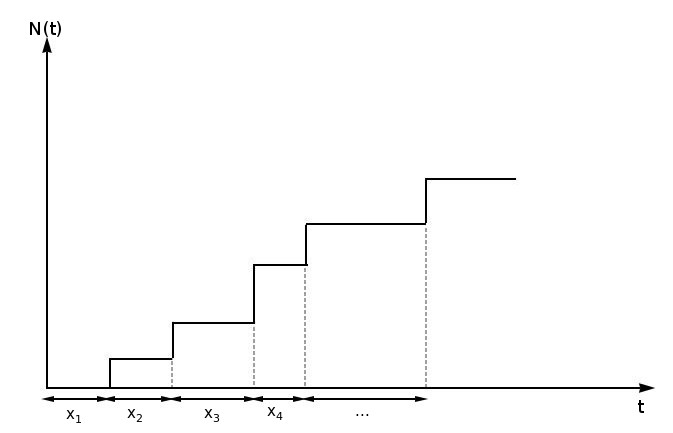
\includegraphics[width=0.7\textwidth]{img/renewal.jpg}
		\caption{Representation of a Renewal process}
	\end{figure}

	where
	\begin{itemize}
		\item $ S_n = W_n = \sum\limits_{k=1}^n X_k =$ time of the n-th renewal
		\item $ N(t) = $ number of events in $(0, t] = \max\,\{n : W_n \le t \}$
	\end{itemize}

	Since all variables are indipendent from the past, the knowledge of $N(t)$ or $W_n$ allows to fully characterize the process.

\subsection{Renewal function}
	Given a serie of renewals, it can be interesting to obtain the probability distribution on the \emph{n}-th event: since it describes a sum of i.i.d. r.v., it is the \emph{n}-th convolution of $F(x)$ with itself.

	\begin{equation}
		F_n(t) = \prob[W_n \le t] \stackrel{(*)}{=} \prob[N(t) \ge n]
	\end{equation}
	where (*) holds for $W_n$ definition.

		\begin{definition}[Renewal function]
			The sum over $n$ of these probabilities gives the expected number of renewals at time $t$, defined as $M(t)$ and called \emph{renewal function}.

			\begin{equation}
				M(t) = \exp[N(t)] = \sum\limits_{k=1}^{+\infty}\prob[N(t)\ge k] = \sum\limits_{k=1}^{+\infty} F_k(t)
			\end{equation}
		\end{definition}

\subsection{Time intervals}
	Other parameters of interest are the times of the renewals that are close to a time instant $t$, that is used to split the inter-renewal time.

	\begin{equation} \begin{cases}
		\delta_t = t - W_{N(t)} & \rightarrow
			\text{~~current life (or age)} \\
		\gamma_t = W_{N(t)+1}-t & \rightarrow
			\text{~~residual lifetime} \\
		\beta_t = \delta_t + \gamma_t & \rightarrow
			\text{~~total lifetime}
	\end{cases} \end{equation}

	\bigbreak
	An interesting result can be proven for Poisson processes with intensity $\lambda$.
	In this case, given $\beta_t = \delta_t + \gamma_t$, the joint distribution of $\delta_t$ and $\gamma_t$ can be written as follows.

	\begin{equation}
		\prob[\gamma_t > x, \delta_t > y ] =
		\begin{cases}
			e^{-\lambda \cdot (x+y)} & \text{if } y < t \\
			0 & \text{if } y \ge t \\
		\end{cases}
	\end{equation}
	where the second case takes into account that the previous event can not happen before time 0.

	The expectation of $\beta_t$ can be computed naturally as
	\begin{equation*}
		\exp[\beta_t] = \exp[\gamma_t] + \exp[\delta_t] =
		\frac{1}{\lambda} + \exp[\delta_t] =
		\frac{1}{\lambda} + \int_0^t e^{-\lambda \cdot x} dx =
		\frac{2-e^{-\lambda \cdot t}}{\lambda}
	\end{equation*}
	where again it is taken into account that $\delta_t$ must be smaller than $t$, i.e. the last renewal cannot happen before 0.

	The asymptotic behaviour of this parameter, that gets rid of the transient component, gives this surprising result.
	\begin{equation*}
		\lim_{t \to +\infty} \exp[\beta_t] = \lim_{t \to +\infty} \frac{2-e^{-\lambda \cdot t}}{\lambda} = \frac{2}{\lambda} > \frac{1}{\lambda} = \exp[X] \text{ where } X \sim exp(\lambda)
	\end{equation*}
	This result is indeed correct, but it clashes with our previous knowledge of the mean interarrivals time $X$ for Poisson process.
	This paradox is easily explained with the concept of \emph{picking bias}: the choice of a random observation instant $t$ changes the statistical behaviour of the time interval, since bigger ones are privileged.

\section{Asymptotic results}
\begin{theorem}[Ross p. 101 and passim]
	Given a renewal process made of a sequence $X_k$ i.i.d. r.v., we can state that, with probability 1,
	\begin{numcases}{}
		\lim_{t \to +\infty} N(t) = N(\infty) = +\infty \label{eq:nt_to_infty} \\
		\lim_{n \to +\infty} \frac {S_n} {n} =
			\exp[X] <+\infty\quad \label{eq:renewal_partial_sum} \\
		\lim_{t \to +\infty} \frac{N(t)}{t} = \frac{1}{\mu} \label{eq:nt_grows_linearly}
	\end{numcases}
\end{theorem}
% In essence this results states that in finite time we have a finite number of renewals. Viceversa in infinite time we have infinite renewals.

\begin{proof}
	\proofpart (equation \eqref{eq:nt_to_infty})

	In have infinite time, we have a finite number of renewals if and ony if there exists an event that is the last one, i.e. its assiciated renewal time $X_k$ takes an infinite amount of time.
	\begin{equation*}
		\begin{split}
			\prob[N(\infty)<\infty] &= \prob[X_n = \infty \text{ for some n}] = \prob \left[ \bigcup\limits_{n=1}^{+\infty}\{X_n = \infty \} \right] \\
			&\le \sum\limits_{n=1}^{+\infty}\prob[X_n = \infty] = 0 \text{~because~} F(\infty)=1
		\end{split}
	\end{equation*}

	\proofpart (equation \eqref{eq:renewal_partial_sum})

	By $S_n$ definition, we have that $ S_{N(t)} / N(t)$ is the average interarrival time for the first $N(t)$ renewals and so for the \emph{Strong Law of Large Numbers} we have that this time average converges to the expectation.
	$$ \lim_{t \to +\infty} \frac{S_{N(t)}}{N(t)} = \lim_{t \to +\infty} \frac{S_{N(t)+1}}{N(t)+1} = \lim_{N \to +\infty} \frac{S_{N}}{N} = \mu $$

	\proofpart (equation \eqref{eq:nt_grows_linearly})

	By $S_n$ and $N(t)$ definitions, we have that $S_{N(t)}$ and $S_{N(t)+1}$ are respectively the time of the last and the next renewal of a given time $t$.

	\begin{equation*}
			S_{N(t)} \le t < S_{N(t)+1} \implies
			\frac{S_{N(t)}}{N(t)} \le \frac{t}{N(t)} < \frac{S_{N(t)+1}}{N(t)} =\frac{S_{N(t)+1}}{N(t)+1} \cdot \frac{N(t)+1}{N(t)}
	\end{equation*}

	Finally, for the sandwich theorem and for equation \eqref{eq:renewal_partial_sum}, we have that
	$$ \mu \le \lim_{t \to +\infty} \frac{t}{N(t)} \stackrel{(*)}{\le}\mu \quad \implies \lim_{t \to +\infty} \frac{t}{N(t)} = \mu $$
	Where in $(*)$ the strict $<$ became $\le$ as we were dealing with limits.
\end{proof}


\begin{theorem}[K.T. page 102]
	We will now prove some interesting properties of the renewal function $M(t)$.

	\begin{numcases}{}
		\lim_{n \to +\infty} F_n(t) = 0 \text{ at least geometrically} \label{eq:Fn_geometric_decreasing} \\
		\forall t, \, M(t) < +\infty \label{eq:mt_always_finite} \\
		\lim_{t \to +\infty} M(t) = +\infty \label{eq:mt_diverges}
	\end{numcases}

\end{theorem}
\begin{proof}
	\proofpart (equation \eqref{eq:Fn_geometric_decreasing})
	Considering the distributions of the $r$-th renewal, we can state that

	\begin{equation}
		\exists r > 0: F_r(t) = \prob[S_r \le t] = \prob \left[ \sum_{i=1}^r X_i \le t \right] < 1
	\end{equation}

	Conversely, we can show that

	\begin{equation} \begin{split}
		\forall t, \exists r: ~ \prob[S_r > t] & = \prob \left[ \sum_{i=1}^r X_i > t \right]
			\ge \prob \left[ X_k > \frac{t}{r} \,\forall k=1, \ldots, r \right] = \\
		& = \left( \prob \left[ X_k > \frac{t}{r} \right] \right) ^ r =
			\left( 1 - F \left( \frac{t}{r} \right) \right) ^ r > 0
	\end{split} \end{equation}

	Thus we have proved that $ \lim_{n \to +\infty} F_r(t) = 0 $ at least geometrically.

	\proofpart (equation \eqref{eq:mt_always_finite} and \eqref{eq:mt_diverges})
	First we derive a nice property of $F_n(t)$ distributions that holds for every $m \in [1,\, n-1]$:

	\begin{equation} \label{eq:fn_upper_bound}
		\begin{split}
			F_n(t) &= \int\limits_0^t F_{n-m}(t-\xi) dF_m(\xi) \quad\\
			& \le \int\limits_0^t F_{n-m}(t) dF_m(\xi) \le F_{n-m} \cdot F_m(t)
		\end{split}
	\end{equation}

	We will use this property to set an upper bound for $M(t)$, as follows

	\begin{equation} \label{eq:mt_convergence}
		\begin{split}
			M(t) &= \exp[N(t)] = \sum\limits_{j=1}^{+\infty} F_j(t) = \sum\limits_{n=0}^{+\infty} \sum\limits_{k=1}^{r} F_{n r + k}(t) \le \\
			& \stackrel{(1)}{\le} \sum\limits_{n=0}^{+\infty} \sum\limits_{k=1}^{r} F_r(t) \, F_{(n-1) r + k}(t) \le \\
			& \stackrel{(1)}{\le} \sum\limits_{n=0}^{+\infty} \sum\limits_{k=1}^{r} F_r(t) \left[ F_r(t) \, F_{(n-2) r + k}(t) \right] = \\
			& = \sum\limits_{n=0}^{+\infty} \sum\limits_{k=1}^{r} F^2_r(t) \, F_{(n-2) r + k}(t) \le \ldots \stackrel{(2)}{\le} \sum\limits_{n=0}^{+\infty} F^n_r(t) \sum\limits_{k=1}^{r} F_k(t)
		\end{split}
	\end{equation}
	where
	\begin{itemize}
		\item[(1)] both hold by applying equation \eqref{eq:fn_upper_bound}
		\item[(2)] is obtained applying \eqref{eq:fn_upper_bound} recursevely
	\end{itemize}

	While the latter term on $k$ is always finite, since it is a finite sum, the former converges only if the $F_r(t)$ terms converge at least geometrically.

	The two thesis are then proved.

	\begin{equation}
		\begin{dcases}
			M(t) \le \sum\limits_{n=0}^{+\infty} F^n_r(t) \sum\limits_{k=1}^{r} F_k(t) < + \infty & \text{for finite } t \\
			M(t) = +\infty & \text{ for } t \to +\infty
		\end{dcases}
	\end{equation}
	where the latter holds since
	$$ \lim_{t \to +\infty}M(t) = \lim_{t \to +\infty} \sum\limits_{j=1}^{+\infty} F_j(t) = +\infty \text{ since } \lim_{t \to +\infty} F_j(t) = 1 $$
\end{proof}

\section{Renewal argument}

% \begin{definition}[Convolution]
% 	For any monothonic function $A$ and for any well behaved function $B$ we define the convolution as
% 	\begin{equation}\begin{split}
% 		A \ast B &= \int\limits_0^t B(t-\eta)\cdot dA(\eta) = B \ast A \\
% 		% & \implies \int a(t-x)\cdot dM(x) = M \ast a ~(t)
% 	\end{split}\end{equation}
% \end{definition}

% \begin{remark}[Expectation as convolution]
% 	We can observe that, for continue random variables, the expectation is a convolution that deals with probability distributionss.
% 	$$ \exp[a(t-X)]=\int a(t-x)\cdot dF(x) $$
% \end{remark}

The \emph{renewal argument} is less a proved result than a way of solve problems during the analysis of renewal processes.

It consists of conditioning on the first renewal and then build a recursive equation on the quantity of desire. For example, to compute $M(t)$ one could proceed as follows.

\begin{equation}
	\exp[N(t)| X_1 = x] =
	\begin{cases}
	0 & x>t \\
	1+M(t-x) & x \le t
	\end{cases}
\end{equation}
where in the first case the renewal has yet to happen, while in the second it is counted and the quantity $M$ is computed on the remaining time.

Averaging on the first event distribution, we can get the unconditioned value of $M(t)$:
\begin{equation} \label{eq:mt_renewal_equation}
	\begin{split}
	M(t)= \exp[N(t)]&=\int\limits_0^{+\infty}\exp[N(t)|X_1=x] \cdot dF(x)\\
	&=\int\limits_0^{t}[1+M(t-x)] \cdot dF(x)\\
	&= F(t) + \int\limits_0^{t}M(t-x) \cdot dF(x)\\
	&= F(t) + F \ast M ~ (t)
	\end{split}
\end{equation}

\section{Renewal equations}

\begin{definition}[Renewal Equation]
	Formulas like \eqref{eq:mt_renewal_equation} are so often encountered in these field of study that they took the name of \emph{renewal equations}.

	\begin{equation} \label{eq:renewal_equation}
			A(t) = a(t) +\int\limits_0^{t}A(t-x) \cdot dF(x)
	\end{equation}
	with $a(t)$ given and $F(x)$ a probability distribution.

	Setting $a(t) = F(t)$ and $A(t) = M(t)$ we obtain the equation \eqref{eq:mt_renewal_equation}.
\end{definition}

\begin{theorem}[4.1 K.T. p.184]
	Let a(t) be a bounded function, the renewal equation has an unique solution $A(t)$ bounded on finite intervals, that is
	\begin{equation} \label{eq:renewal_solution}
		A(t) = a(t) + \int\limits_0^{t} a(t-x) ~ dM(x)
	\end{equation}
\end{theorem}
In other words it exists an unique solution that doesn't diverge in a finite time.
\begin{proof}
	The proof is in three steps: boundness, existence and uniqueness.
	\proofpart of boundness \label{req:boundness}

	For the triangle inequality and integral properties, we have that
	$$ |A(t)| \le |a(t)| + \int\limits_0^{t}|a(t-x)| \cdot dM(x) $$

	We can easily assess this upper buond for the value of $A(t)$, that proves our thesis.
	\begin{equation}\begin{split}
		\sup_{0\le t \le T} |A(t)| & \le \sup_{0\le t \le T} |a(t)| + \int\limits_0^{T}\sup_{0\le \eta \le T}|a(\eta)| \cdot dM(x) \\
		& = \sup_{0\le t \le T} |a(t)| \cdot [ 1+M(T) ] < \infty \text{ as }
		\begin{cases}
			|a(t)| \text{ is bounded for hypothesis} \\
			M(t) < \infty \text{ for } t<\infty
		\end{cases}
	\end{split}\end{equation}

	\proofpart of existence

		We will now assess that our guess is actually a valid solution obtaining \eqref{eq:renewal_equation} from \eqref{eq:renewal_solution}.

		\begin{equation}\begin{split}
			A(t) &= a(t) + M \ast a(t) = a(t) + \left(\sum\limits_{k=1}^{+\infty} F_k \right) \ast a(t) = \\
			&= a(t) + F \ast a(t) +\left(\sum\limits_{k=2}^{+\infty} F_k \right) \ast a(t) = \\
			&= a(t) + F \ast a(t) +\left(\sum\limits_{k=2}^{+\infty} F \ast F_{k-1} \right) \ast a(t) = \\
			&= a(t) + F \ast \left[ a(t) + \left(\sum\limits_{k=1}^{+\infty} F_k \right) \ast a(t) \right] = \\
			&= a(t) + F \ast \left[ a(t) + M(t) \ast a(t) \right] = \\
			&=a(t) + F \ast A ~ (t)
		\end{split}\end{equation}

	\proofpart of uniqueness

	This proof is the inverse reasoning of the proof of existence, as we will obtain \eqref{eq:renewal_solution} from \eqref{eq:renewal_equation}.

	\begin{equation}\begin{split}
		A(t) &= a(t) + F \ast A(t) \quad \text{which is a recursive expression.} \\
		&= a(t) + F \ast \left[a(t) + F \ast a(t) \right] = a(t) + F \ast a ~ (t) + F_2 \ast a(t) \\
		&= a(t) + F \ast a ~ (t) + F_2 \ast \left[a(t) + F \ast a(t) \right] \\
		&= a(t) + F \ast a(t) + F_2 \ast a(t) + F_3 \ast a(t) = \dots  = \\
		&= a(t) + \left( \sum\limits_{k=1}^{n-1}F_k\right) \ast a(t) + F_n \ast a(t) \\
	\end{split} \end{equation}

	For $n \to +\infty$, the term between parenthesis becomes $M(t)$, for its definition.
	\begin{equation}
		A(t) = a(t) + M \ast a(t) + \lim_{n \to +\infty} F_n \ast a(t)
	\end{equation}

	For our proof we will show that the remaining limit goes to zero.
	\begin{equation} \begin{split}
		|F_n \ast a(t)| & = \left| \int\limits_0^{t}A(t-\eta) \cdot dF_n(\eta) \right| \le \\
		& \le \int\limits_0^{t}|A(t-\eta)| \cdot dF_n(\eta) \le \sup\limits_{0 \le \eta \le t} |A(\eta)| \cdot F_n (t)
	\end{split}\end{equation}

	Since $A(\eta)$ is bounded (see part \ref{req:boundness}) and $F_n(t)$ is infinitesimal in $n$, the proof is completed.
\end{proof}

\section{Wald's equation}

Let's now apply the renewal equation to another relevant quantity of a renewal process: we focus on the expectation of the next arrival time after a given time $t$.
	$$ S_{N(t) + 1} = \sum\limits_{i=1}^{N(t)+1}X_i $$

This resembles a random sum, but it is not the case, since $N(t) + 1$ is not independent on the various $X_i$.

With the knowledge acquired on renewal processes, we try to answer this question applying the renewal argument on $ A(t) = S_{N(t)+1} $, discerning again between times $t$ before and after first event.

\begin{equation}\begin{split}
	\exp[A(t)|X_1=x] &=
	\begin{cases}
		x & x>t \\
		x + A(t-x) & x \le t
	\end{cases}
\end{split} \end{equation}

Thus we can build a renewal equation.

\begin{equation} \begin{split}
	A(t) &= \int\limits_0^{+\infty} \exp[S_{N(t)+1}|X_1 = x] \cdot dF(x) \\
	&= \int\limits_0^{t} [x+ A(t-x)] \cdot dF(x) + \int\limits_t^{+\infty} x \cdot dF(x) \\
	&= \int\limits_0^{+\infty} x \cdot dF(x) + \int\limits_0^{t} A(t-x) \cdot dF(x) \\
	&= \exp[X_1] + \int\limits_0^{t} A(t-x) \cdot dF(x)\\
\end{split}\end{equation}

As proved earlier, the final solution for $A(t)$ is
$$ \exp[S_{N(t)+1}] = A(t) = \exp[X_1] + \int\limits_0^{t} \exp[X_1] \cdot dM(x) = \exp[X_1]\cdot [1+M(t)] $$
where the expectation is bounded if $\exp[X_1]$ is finite.

This is the same result we would have obtained with the formula of the random sum: this gives us the idea of extending random sums theory with the concept of \emph{stopping time}.

\begin{definition}[Stopping Time]
An integer random variable N is called \gls{st} for the i.i.d. sequence $X_i$ if
\begin{equation}
	\forall i > n, \{N=n\} \text{ is independent of }X_i
\end{equation}

Less formally, N is independent on what happens after $X_n$.
\end{definition}

\begin{theorem}[Wald's equation]
	Let $X_1, X_2, \dots, X_N $ be an i.i.d. sequence with finite mean and N a stopping time such that $\exp[N] < \infty$. Then

	\begin{equation}
		\exp\left[\sum\limits_{n=1}^N X_n \right] = \exp[N] \cdot \exp[X]
	\end{equation}
\end{theorem}
---
\begin{proof}
	We are gonna use a trick that will allow us to write the random sum as an infinite sum. \\

	Let $I_n = \begin{cases} 1 & N \ge n \\ 0 & N<n \end{cases}$~, we can observe immediatly that
	$$ \{I_n=1\} = \{N \ge n \} = \bigcap\limits_{i=1}^{n-1}\{ N \neq i \} \implies \{I_n=1\} \perp X_n, X_{n+1}, \ldots $$

	% it is independent on the future of $X$ after $n$.
	Now the proof of the thesis is straightforward.
	\begin{equation}\begin{split}
		\exp\left[\sum\limits_{n=1}^{N}X_n\right] &= \exp\left[\sum\limits_{n=1}^{N}X_n \cdot I_n \right] \stackrel{(1)}{=} \sum\limits_{n=1}^{+\infty}\exp[X_n \cdot I_n] \stackrel{(2)}{=} \\
		&=\sum\limits_{n=1}^{+\infty}\exp[X_n] \cdot \exp[I_n] \stackrel{(3)}{=} \exp[X]\cdot\sum\limits_{n=1}^{+\infty}\exp[I_n] \stackrel{(4)}{=} \\
		&= \exp[X] \cdot \sum\limits_{n=1}^{+\infty}\prob[N \ge n] = \exp[X] \cdot \exp[N]
	\end{split}\end{equation}
	where
	\begin{itemize}
		\item[(1)] holds since the sum converges always, since it is actually a finite one
		\item[(2)] holds because of the indipendence between $I_n$ and $X_n$
		\item[(3)] is due to the identically distributed $X_k$
		\item[(4)] holds for $I_n$ definition
	\end{itemize}
\end{proof}

\subsection{Examples}
	\begin{enumerate}
		\item Given $\prob[X_i=0]=\prob[X_i = 1] = \frac{1}{2}$, $N = \min\{n : X_1 + \dots + X_N =10\}$ is a \gls{st}, and in particular
		$10 = \exp[N] \cdot \exp[X] = 0.5 \cdot \exp[N] \implies \exp[N]=20$
		\item Given $\prob[X_i=-1]=\prob[X_i = 1] = \frac{1}{2}$, $N = \min\{n : X_1 + \dots + X_N =1\}$ is a \gls{st}, but the expected stop time
		is $1 = \exp[N] \cdot \exp[X] = 0 \cdot \exp[N] $, which is an absurd.

		We conclude that Wald's equation doesn't apply and so it must be that $N$ has not finite mean: $\exp[N]=+\infty$
	\end{enumerate}

	\section{Elementary renewal theorem}
	Let's take the limit
	\beq
	\lim_{t \to \infty}\frac{M(t)}{t} = \frac{1}{\mu}
	\eeq
	where $\mu = E[X]$.\\
	Then we can prove that $\frac{M(t)}{t} = E[\frac{N(t)}{t}]$ and that $\lim_{t \to \infty}\frac{M(t)}{t} = \frac{1}{\mu}$ w.p. 1.
	\subsubsection{Counter example}
	Let $U$ be a uniform r.v. $U(0,1)$ and let $Y_n$ be a r.v. such that:
	\beq
	Y_n =
	\begin{cases}
	0 \quad for \quad U \ > \frac{1}{n}\\
	n \quad for \quad U \leq \frac{1}{n}
	\end{cases}
	\eeq
	Where the second equation brings to the espressions $\frac{M(t)}{t} > \frac{1}{\mu} - \frac{1}{t}$ and $\lim_{t \to \infty} \frac{M(t)}{t} \geq \frac{1}{\mu}$

	\textbf{NOTE}: In the book the notation has also the expression \textit{"lim \textbf{inf}"} since, in this way, the demonstration is "easier" to do, in fact we can also see graphically that the $inf$ expression guarantees that we have a lower bound. Figure\ref{fig:graph1}
	\begin{figure}[h]
	\centering
	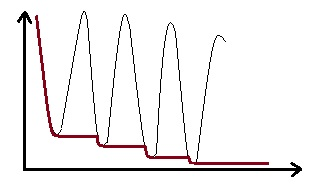
\includegraphics[width=0.5\textwidth]{Cri_graph1.jpg}
	\caption{lower bound}
	\label{fig:graph1}
	\end{figure}
	Now the other bound must be proved, so to reach the equality, but here there is a problem: $S_{N(t)}$ is not known, so it is difficult to demonstrate the inequality $t \geq S_{N(t)}$ since I cannot take the expectation. So we use a \textbf{trick}: we consider a new renewal process obtained by the previous one by truncation:
	\begin{equation}
	X_i^c =
	\begin{cases}
	X_i \qquad X_i \leq c\\
	c \qquad X_i >c
	\end{cases}
	\end{equation}

	What do we have for this truncated process?\\
	First of all we have the relations:
	\begin{equation}
	\begin{split}
	N^c(t) \geq N(t)\\
	M^c(t) \geq M(t)
	\end{split}
	\end{equation}
	because, since events are spaced by numbers that are no bigger, times are no smaller.\\

	So for the truncated process we have $t \geq S_{N^c(t) +1}$ (in the truncated process, the $X$ I'm adding cannot be bigger than $c$), and the next inequality also goes:
	\begin{equation}
	c+t \geq S_{N^c(t)+1}
	\end{equation}•
	If now I take this inequality expectation I obtain:
	\begin{equation}
	t+c \geq \mu^c(1+M^c(t))
	\end{equation}•
	and since $M^c(t) \geq M(t)$ from the previous inequality, I can say that:
	\begin{align}
	\begin{split}
	\mu^c(1+M^c(t)) \geq \mu^c(1+M(t))\\
	\frac{M(t)}{t} \leq \frac{1}{\mu^c} \frac{1}{t}(\frac{c}{\mu^c}-1) \qquad \forall c > 0 \quad (valid\quad for\quad any\quad truncation)
	\end{split}
	\end{align}

	NOTE: $c$ is an index, not an exponent.
	So now I take the limit:
	\beq
	\lim_{t \to \infty} sup \frac{M(t)}{t} \leq \frac{1}{\mu^c} \qquad \forall c > 0
	\eeq
	Since it is true $\forall c$ , it is true also for $c \to \infty$ (which means that truncation becomes less an less important until I don't truncate at all), so I obtain:
	\beq
	\lim_{t \to \infty} sup \frac{M(t)}{t} \leq \lim_{c \to \infty} \frac{1}{\mu^c}
	\eeq
	where $\mu^c = \int_0^c(1-F(x))\,dx$, so as $c \to \infty$ we see that $\mu^c \to \mu = \int_0^\infty(1-F(x))\,dx$. See figure\ref{fig:mu}
	\begin{figure}
	\centering
	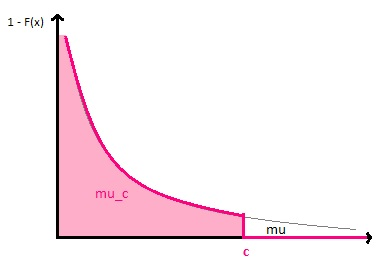
\includegraphics[width = 0.5\textwidth]{Cri_mu.jpg}
	\caption{This graph is the complementary distribution of $X^c$}
	\label{fig:mu}
	\end{figure}
	So at the end we conclude that
	\beq
	\lim_{t \to \infty} sup \frac{M(t)}{t} \leq \lim_{c \to \infty} \frac{1}{\mu^c} = \frac{1}{\mu}
	\eeq
	\\
	\textit{cvd}
	\subsection*{Observation}
	In the book, at the beginning, they assume that $E[X] < \infty$. Reasoning on it we can observe that:
	\begin{itemize}
	\item In the first part is not needed;
	\item In the second one, even though $\mu = 0$, I can make it finite by truncation;
	\end{itemize}
	\subsection{Two important results proofs}
	We now proceed with proving two important results:
	\begin{itemize}
	\item \textbf{1}: $E[S_{N(t)+1}] = (1+M(t))E[X]$;
	\item \textbf{2}: $E[S_{N(t)}] \ne M(t)E[X]$;
	\end{itemize}
	In the first case there is no case in which the equality is not true, so we can state that this equality is always true; in the second case there is a non-zero number of cases in which the equality is not true, and so it cannot taken as true in general.
	\subsubsection*{$1^{st}$ Statement}
	In this case represents a Poisson process: $S_{N(t)+1} = t + \gamma_t$ and $S_{N(t)} = t - \delta_t$;\\
	If i sit at time $t$, then $\gamma_t$ is the time until the next renewal, which means that the time until the next renewal occurs is $t + \gamma_t$, and so this is why $S_{N(t)}$ is the instant $t$ minus the time since the last renewal occurred $\delta_t$. And that's actually true for any renewal process.\\
	Moreover we know that both $\gamma$ and $\delta$ are exponentially distributed (because of Poisson process theory and the memoryless condition of the process): $\gamma_t$ is exponential with parameter $\lambda$, while $\delta_t$ is exponential with parameter $\lambda$ truncated at $t$.\\
	So we can find all the quantities involved:%min 25:00
	\beq
	E[S_{N(t)+1} = t + \frac{1}{\lambda}] \qquad E[S_{N(t)}] = t - \frac{1-e^{-\lambda t}}{\lambda}
	\eeq
	with $M(t) = \lambda t$ and $E[X] = \frac{1}{\lambda}$.\\
	Thanks to it we can see that the equality in true.
	\subsubsection*{$2^{nd}$ Statement}
	In this case we take:
	\beq
	X_i =
	\begin{cases}
	1 \qquad w.p. p\\
	a \geq 2 \qquad w.p. 1-p
	\end{cases}
	\eeq
	How many arrivals do we count?
	\beq
	N(t) =
	\begin{cases}
	1 \qquad w.p. p\\
	0 \qquad w.p. 1-p
	\end{cases}
	\eeq
	And how much time do we count?
	\beq
	S_{N(t)}=
	\begin{cases}
	1 \qquad w.p. p\\
	0 \qquad w.p. 1-p
	\end{cases}
	\eeq
	NOTE: Even though the value is the same, they do not represent the same thing.\\
	What about $S_{N(t)+1}$? $a>t$ so:
	\beq
	S_{N(t)+1} =
	\begin{cases}
	a \quad \text{w.p. $ (1-p)$}  \rightarrow \text{it means it the first renewal}\\
	2  \quad \text{w.p.  $p^2$}  \rightarrow \text{if the first  X is 1 and also the second}\\
	1+a \quad \text{w.p. $ p(1-p)$} \rightarrow \text{if the first X is 1 and the second is a}\\
	\end{cases}
	\eeq
	So:
	\beq
	\begin{split}
	E[S_{N(t)+1}] & = a(1-p)+2p^2+(1+a)p(1-p)\\
	                        & = p^2 + p + (1-p^2)a\\
	\end{split}
	\eeq
	\beq
	\begin{split}
	E[S_{N(t)}] & = p\cdot1 + 0\cdot(1-p)\\
		         & = p E[N(t)] = M(t)\\
		         & =  p\cdot1 + (1-p)\cdot0 = p
	\end{split}
	\eeq
	So I can try those equalities by multiplying
	\beq
	E[N(t)+1]E[X] = (1+p)(p+a(1-p)) = p^2+p+(1-p^2)a = E[S_{N(t)+1}]
	\eeq
	On the other hand:
	\beq
	E[N(t)]E[X] = p(p+(1-p)a) \ne p
	\eeq
	$\leftarrow$ {I can always find a value of $a$ that makes the equality not true}
	So the first equation was found to be true in both cases and it's contrary for the second.
	\subsection{Exercises}
	\subsubsection*{Ex 2.4}
	Each specific error is found on a specific case w.p. $\frac{1}{600}$ so the number of errors on given page is a binomial r.v. $(240,\frac{1}{600})$. At the same time, though, we know that when we have a Bin where $p$ is small and $M$ is big we can approximate it to a Poisson r.v. $\sim P(\frac{240}{600})$, where $\lambda = \frac{240}{600}  \simeq 0.4$.\\
	So I represent the book as:
	\begin{figure}[h]
	\centering
	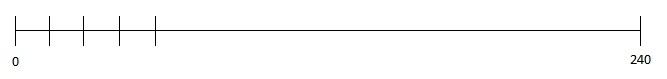
\includegraphics[width = 0.6\textwidth]{Cri_book.jpg}
	\label{fig:book}
	\end{figure}
	Easy to find the probability of what happens i different pages: each page is an independent interval, so:
	\beq
	P[\text{0 errors in 3 pages}\footnote{not necessarily consecutive}] = e^{-1.2}
	\eeq
	\subsubsection*{Ex 2.5}
	We have $N$ points equally distributed in a circle of radius $r$. The distribution of points in the circle of radius $1$ as $N \to \infty$ and $r \to \infty$ is:
	\beq
	\frac{N}{\pi r^2} < \lambda
	\eeq
	While the probability \textit{Prob[points inside r = 1]} is:
	\beq
	\frac{Small_{Area}}{Big_{Area}}
	\eeq
	This bring us to say that \textit{P[a given point is inside r $\leq$ 1] = } $\frac{Area(1)}{Area(r)} = \frac{1}{r^2}$.\\
	The number of points present in the smaller circle is a binary r.v. $\sim bin(N,\frac{1}{r^2})$, so its expected value is:
	\beq
	\text{E[number of points inside the smaller circle]} = \frac{N}{r^2} = \lambda\pi
	\eeq
	where $\lambda$ is the density of points and $\pi$ is the area of unitary circle.\\
	So we have two parameters, the product of which is still constant.
	\begin{align}
	\begin{split}
	N \to \infty \qquad r \to \infty\\
	\frac{N}{\pi r^2} = \lambda' \rightarrow P_{0i}(\lambda\pi)
	\end{split}
	\end{align}
	\subsubsection*{Ex 3.6}
	For $i = 1 \dots n$ I have an indep. PP $\rightarrow X_i(t)$ is an i.i.d. PP($\lambda$).\\
	The problem asks to find the first time such that there is at least one event  in every process, see figure\ref{fig:3.6}
	\begin{figure}[h]
	\centering
	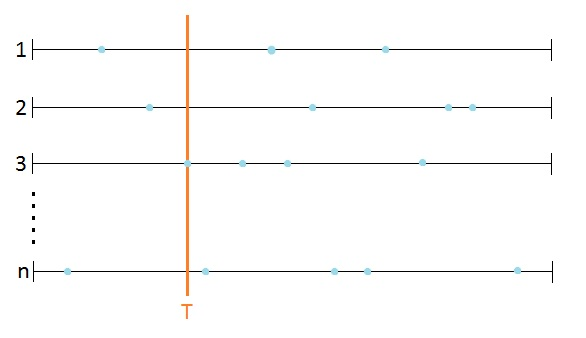
\includegraphics[width =0.6\textwidth]{Cri_Ex3_6.jpg}
	\label{3.6}
	\end{figure}
	Since the process is Poisson, we have that $P[T\leq t] = 1-P[0 events] = 1-e^{-\lambda t}$ for one process, while for $n$ processes we have $P[t \leq t] = (1-e^{}-\lambda t)^n$.\\
	We could actually see the problem from a different point of view: this view counts the events in the Poisson Poisson process and uses the independence to find the probability that none of them has seen $0$ events.\\
	So we can see how we can look at $T$: we get that $T$ is the time at which the last process has its first event and it will be the biggest value among the exponentials; the first event will occur, obviously, with exponential time, so using this reasoning we can express the r.v. $T$ as:
	\beq
	T = \max_{i = 1,2,\dots,n}{exp_i(\lambda)}
	\eeq
	So I can turn the point into a question: what is the distribution of the maximum among the i.i.d variables?
	\begin{align}
	\begin{split}
	P[max{X_1,X_2,\dots,X_n} \leq t] & = P[X_i \leq t, \quad i = 1,2, \dots, n]\footnote{since the X's are i.i.d.}\\
						  & = (P[X \leq t])^n = (1-e^{-\lambda t})^n
	\end{split}
	\end{align}
	In general this shows that if we take $F_{max}(t)$, then $F_{max}(t) = (F(t))^n$; on the other side:
	\begin{align}
	\begin{split}
	P[min{X_1,X_2,\dots,X_n} >t ] & = P[X_i > t \forall i = 1,2,\dots, n] \\
					        & = (P[X > t])^n
	\end{split}
	\end{align}
	So we found that $1-F_{min}(t) = (1-F(t))^n \rightarrow F_{min}(t) = 1- (1-F(t))^n$
	\subsubsection*{Problem 3.6}
	Service facility situation: service when $Q$ users arrived $\rightarrow$ a process that focuses on the $q^{th}$ arrival in sequence.\\
	$T = $ service time.
	\begin{figure}
	\centering
	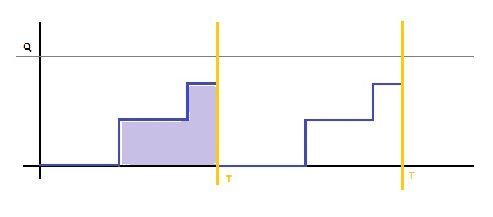
\includegraphics[width = 0.6\textwidth]{Cri_scale.jpg}
	\caption{Prob 3.6}
	\end{figure}
	We have to show that $E[\int_{0}^{T}N(t)dt] = \frac{q(Q-1)}{2\lambda}$; The first question is intuitive: we can see that if the time at which a user is served is the time at which the $q^{th}$ user arrives, then I have to wait for $q$ users to arrive to be served.\\
	I then have to take the expectation of the blue area, to do it I can use two different approaches: I can look how much time each user has to wait and then I sum all of then (and that corresponds to summing the horizontal slices of the area), or I can look at it vertically and see how much time there is one, two, three users waiting and then multiplying this amount of time by the number of users who are waiting during that time.\\
	So with the first approach:
	\begin{itemize}
	\item The first user will have to wait $\frac{1}{\lambda}(Q-1)$ inter-arrival times;
	\item The second user arrives after $2$ inter-arrival times and so he has to wait $\frac{1}{\lambda }(Q-2)$ inter-arrival times;
	\item After the second user more users will arrive until the $q^{th}$ user will arrive, and for it the waiting time will be $0$;
	\end{itemize}
	So the average sum of all the waiting time is the constant $1/\lambda$ times  the sum of the first $Q-1$ integers: $\frac{1}{\lambda}[(Q-1)+(Q-2)+\dots+1]$.\\
	With the second approach we see that:
	\begin{itemize}
	\item At the beginning no one is waiting in line;
	\item After the first arrival $1$ user is waiting;
	\item After the second arrival $2$ users are waiting;
	\item After the $(q)^{th}$ arrival, $Q-1$ users are waiting and so the structure is the same as previously.
	\end{itemize}
	\subsubsection*{Ex 4.1}
	Given $n$ arrivals, we take the quantity $E[w_1] = \int_{0}^{1}(1-t)^n dt = \frac{1}{n+1}$ where $w_1$ is the smallest among $n$ i.i.d. uniform r.v. between $0$ and $1$ and so the distribution is the distribution of the minimum of $n$ i.i.d. uniform r.v., and its complementary distribution is the $n^{th}$ power of the complementary distribution.\\
	\subsubsection*{Ex 4.3}
	Suppose we have $5$ arrivals, the cumulative time is the area in figure4, but we know that the arrival times are i.i.d. uniform so each user has to wait average waiting time is $0.5$ hours, so $0.5\times5 = 2.5$.\\
	\subsubsection*{Ex 4.5}
	Here assume we have $\alpha$  and the service time is an exponential r.v. $\sim exp(\alpha)$, and the probability $P[\text{at time 1 h the queue is empty}]$ is estimated considering each user arriving uniformly. So at the end the number of users is binomial and, conditioning on the uniform variable, we get:
	\begin{align}
	\begin{split}
	p = P & [\text{a uniformly arriving user has not left at time 1 h}] =\\
	& P[U_i + Y_i > 1] = \int_{0}^{1}e^{-\alpha(1-u)}du = \frac{1-e^{-\alpha}}{\alpha}
	\end{split}
	\end{align}
	So the probability becomes finding the probability that all users that had arrived here have left: it is the value $(1-P)^{n}$ with $n = $ \textit{number of users}:
	\begin{align}
	P&[\text{System empty at time 1|5 arrivals}] = (1-\frac{1-e^{-\alpha}}{\alpha})^5
	\end{align}
	\begin{figure}[h]
	\begin{minipage}[c]{0.5\textwidth}
	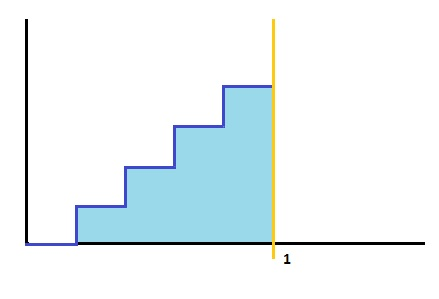
\includegraphics[width = 0.9\textwidth]{Cri_area.jpg}
	\caption{Ex 4.3}
	\end{minipage}
	\hspace{10mm}
	\label{fig:area}
	\begin{minipage}[c]{0.5\textwidth}
	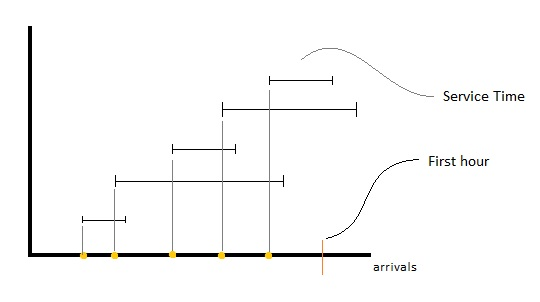
\includegraphics[width = 0.9\textwidth]{Cri_arrivals.jpg}
	\caption{Ex 4.5}
	\end{minipage}
	\end{figure}

\section{The key renewal theorem}
\begin{definition}
	(Point of increase) Given a distribution function F we call \textit{point of increase} every point $\alpha$ such that
	\begin{equation}
		F(\alpha+\epsilon)-F(\alpha-\epsilon)>0 \quad  \forall \quad
		\epsilon > 0
	\end{equation}
\end{definition}
\begin{definition}
	(Arithmetic function) We say that a distribution function F is \textit{arithmetic} if $\exists \lambda > 0$ such that F has points of increase exclusively among the points 0, $\pm \lambda$, $\pm 2\lambda$, \dots .

	We call \textit{SPAN} the largest $\lambda$ for which F is still arithmetic.
\end{definition}

The distribution function of a discrete random variable with possible values 0, 1, 2, \dots is an arithmetic function with SPAN=1.

\begin{definition}
	(Directly Riemann Integrable Function) Given a function g defined on [0, $\infty$) we define the following quantities for $\delta > 0$:
	\begin{align*}
		\underline \sigma (\delta) = \delta \cdot \sum_{n=1}^{\infty} min\{g(t):(n-1)\delta \leq t \leq n \delta \}
		\\
		\bar \sigma (\delta) = \delta \cdot \sum_{n=1}^{\infty}max\{g(t):(n-1)\delta \leq t \leq n \delta \}
	\end{align*}
	We say that g is directly Riemann integrable if both $\underline \sigma (\delta)$ and $\bar \sigma (\delta)$ converge absolutely $\forall \quad \delta > 0$ and if:
	\begin{equation}
		\underline \sigma (\delta) - \bar \sigma (\delta) \rightarrow 0 \quad \delta \rightarrow 0
		\end{equation}
\end{definition}

We note that every function for which $\int_{0}^{\infty} |g(t)| dt$ < $\infty$ (g is absolutely integrable) is directly Riemann integrable.

\begin{theorem}
	(Key Renewal Theorem) It is given a distribution function F of a positive random variable $a$ with mean $\mu$. We suppose that $a$ is directly Riemann integrable and that $A$ is the solution of the \textit{renewal equation}
	\begin{equation}
		A(t)=a(t)+\int_{0}^{t}A(t-x)dF(x)
	\end{equation}
	If F is not arithmetic, then
	\begin{equation*}
		\lim_{t \rightarrow \infty} A(t) =
		\begin{dcases}
			\frac{1}{\mu} \int_{0}^{\infty}a(x)dx \quad & if \quad \mu < \infty \\
			0 \quad & if \quad \mu = \infty
		\end{dcases}
	\end{equation*}
	If F is arithmetic with SPAN = $\lambda$ then, $\forall c > 0$
	\begin{equation*}
		\lim_{t \rightarrow \infty} A(c+n\cdot \lambda) =
		\begin{dcases}
			\frac{\lambda}{\mu} \sum_{n=0}^{\infty}a(c+n \cdot \lambda) \quad & if 	\quad \mu<\infty \\
			0 \quad & if \quad \mu = \infty
		\end{dcases}
	\end{equation*}
\label{KRT1}
\end{theorem}

The theorem \ref{KRT1} can be also expressed in the following form:

\begin{theorem}
	(Key renewal theorem) Is given a distribution function F of a positive random variable with mean $\mu$. We suppose $h>0$ and that $M(t)=\sum_{k=1}^\infty F_{k}(t)$ is the \textit{renewal function} associated with F.
	If F is not arithmetic then
	\begin{equation}
		\lim_{t \rightarrow \infty} [M(t+h)-M(t)]=\frac{h}{\mu}
	\end{equation}
	If F is arithmetic with SPAN = $\lambda$ then:
	\begin{equation}
		\lim_{t \rightarrow \infty} [M(t+h)-M(t)]=\frac{h}{\mu} \quad \forall h = n \cdot \lambda
	\end{equation}
	\label{KRT2}
\end{theorem}

We note that the \textit{elementary renewal theorem} $\lim_{t \to \infty} M(t) / t = 1 / \mu$ is a corollary of the \textit{key renewal theorem} \ref{KRT2}.

\subsection{Application of the key renewal theorem}

\paragraph{Limiting distribution of the excess life}

We say that $\gamma_{t}=S_{N(t)+1}-t$ is the excess life at time t and that $A_z=\prob[\gamma_t>z]$ for a fixed parameter $z>0$.

Conditioning on the first event, we obtain that
\begin{equation*}
	\prob[\gamma_t>z|X_1=x] = \begin{cases}
		1 \quad & if \quad x > t+z \\
		0 \quad & if \quad t+x \geq x > t \\
		A_z(t-x) \quad & if \quad t \geq x > 0
	\end{cases}
\end{equation*}

For the law of the total probability we have
\begin{align*}
	A_z(t) &= \int_{0}^{\infty} \prob[\gamma_t>z|X_1=x] dF(x) = \int_{0}^{t}A_z(t-x)dF(x)+\int_{t+z}^{\infty}dF(x)= \\
	&= \int_{0}^{t}A_z(t-x)dF(x)+ [1-F(t+z)]
\end{align*}

Now we apply the \textit{renewal equation} setting
\begin{equation} \begin{dcases}
	a(t) = 1 - F(t+z) \\
	A_z(t)=\int_{0}^{t} [1-F(t+z-x)] dM(x)+1-F(t+z)
\end{dcases} \end{equation}

\begin{align*}
	\int_{0}^{\infty} a(x) d(x) & = \int_{0}^{\infty}(1-F(x)) d(x) = \\
	& = \int_{z}^{\infty}(1-F(y))dy \leq \int_{0}^{\infty}(1-F(y))dy = \mu
\end{align*}

Supposing $\mu < \infty$, for the \textit{renewal theorem} we obtain that
\begin{equation}
	\lim_{t \rightarrow \infty} \prob[\gamma_t>z] = \lim_{t \rightarrow \infty} A_z(t) = \frac{1}{\mu} \cdot \int_z^{\infty}(1-F(x))dx \quad \forall z > 0
	\label{limitingdistribution}
\end{equation}

From \ref{limitingdistribution} we can determine the limiting distribution for the \textit{current life} $\delta_t$ and for the \textit{total life} $\beta_t$. First we note that
\begin{equation} \label{currtotallife}
	\{\gamma_t \geq x, \delta_t \geq y \}
	\Leftrightarrow
	\{\gamma_{t-y} \geq x+y \}
\end{equation}
From equation \ref{currtotallife} we have that
\begin{align*}
	\lim_{t \rightarrow \infty} \prob[\delta_t \geq y, \gamma_t \geq x] & = \lim_{t \rightarrow \infty} \prob[\gamma_{t-y} \geq x+y] \\ & = \frac{1}{\mu} \cdot \int_z^{\infty}(1-F(z))dz
\end{align*}
In particular we have that
\begin{align*}
	\lim_{t \rightarrow \infty} \prob[\delta_t \geq y] & = \lim_{t \rightarrow \infty} \prob[\delta_t \geq y, \gamma_{t} \geq 0] \\ & = \frac{1}{\mu} \int_z^{\infty}(1-F(z))dz
\end{align*}

So $\frac{1-F(z)}{\mu}$ is the probability density function of $\delta_t$. We are able to compute $\delta_t$ and $\gamma_t$ averages.
\begin{align*}
	\exp[\delta_t]=\exp[\gamma_t] & =\int_z^{\infty} \frac{z}{\mu} (1-F(z))dz \\ & = \frac{z^2}{2\mu} \left( 1-F(z) \right|_0^{\infty} + \int_0^{\infty}\frac{z^2}{2 \mu} f(z)dz= \frac{\exp[X^2]}{2 \exp[X]}
\end{align*}

Finally we conclude that
\begin{equation*}
	\begin{dcases}
		~ \exp[\delta_t] = \frac{\exp[X^2]}{2 \exp[X]} \\
		~ \exp[\gamma_t] = \frac{\exp[X^2]}{2 \exp[X]} \\
		~ \exp[\beta_t] = \frac{\exp[X^2]}{\exp[X]}
	\end{dcases}
\end{equation*}


\paragraph{Asymptotic expansion of the renewal function}
Given a distribution function $F$ of mean $\mu$ and variance $\sigma$ we want to find a more detailed description of the asymptotic behaviour of $M(t)$.

For $t \rightarrow \infty$ we have what follows
\begin{align*}
	M(t)-\frac{t}{\mu} & =\exp[N(t)+1]-\frac{t}{\mu}-1 \\
	& = \frac{1}{\mu} (\exp[S_{N(t)+1}]-t)-1 \\
	& = \frac{1}{\mu} \exp[\delta_t]-1 \\
	& = \frac{1}{\mu}\frac{\exp[X^2]}{2\mu}-1 \\
	& = \frac{\sigma^2+\mu^2}{2\mu^2}-1 \\
	& = \frac{\sigma^2-\mu^2}{2\mu^2}
\end{align*}

Then we finally prove that
\begin{equation}
	\lim_{t \rightarrow \infty} \left( M(t) - \frac{t}{\mu} \right) = \frac{\sigma^2-\mu^2}{2\mu^2}
\end{equation}

\subsection{Delayed renewal processes}
	We assume that $\{X_k\}$ are independent positive random variables but only $X_2,X_3,...$ are identically distribuited.
	In fact $X_1$ has a distribution function $G$ that differs from the distribution function $F$ of the other variables.

	We call such process \textit{delayed renewal process}. Given an ordinary renewal process we can obtain a \textit{delayed renewal process} if we fix the time origin $t=0$ a certain time after the start of the ordinary process.

	Let us put $S_0=0$ and $S_n=X_1+X_2+...+X_n$ and $N(t)$ equal to the number of renewal at time $t$. We must distinguish between the mean number of renewals in the delayed process $M_D(t)$ and the renewal function  $M(t)$ associated to $F$.

	\begin{align}
		& M_D(t) = \exp[N(t)]
		\\ & M(t) = \sum_{k=1}^{\infty}F_k(t)
	\end{align}
	Now we want to prove what follows:
	\begin{align*}
		& \lim_{t \to \infty }\frac{M_D(t)}{t}=\frac{1}{\mu}
		\\ & \lim_{t \to \infty }[M_D(t)-M_D(t-d)]=\frac{d}{\mu}
	\end{align*}

	We have already seen that for a recurrent irreducible aperiodic \gls{mc} the following statament is true.
	\begin{equation}
		\lim_{n \to \infty} P_{jj}^{(n)}=\pi_j=\frac{1}{m_j}=\frac{1}{\sum_{n=1}^{\infty}n \cdot f_{jj}^{(n)}}
	\end{equation}
	Given a recurrent state $j$ we call $N_j(t)$ the number of visits in $j$ by the time $t$. The following statament is always true for any initial state $Y_0$.

	\begin{equation}
		N_j(n)-N_j(n-1)=1 \quad \Leftrightarrow \quad Y_n=j
	\end{equation}

	If $Y_0$ is equal to j, then $N_j$ is a ordinary renewal process. We keep $Y_0=j$ and we obtain what follows.
	\begin{align*}
		& \exp[N_j(n)-N_j(n-1)|Y_0=j]=M(n)-M(n-1)=P_{jj}^{(n)}
		\\ & \Rightarrow \pi_j=\frac{1}{m_j}=\lim_{n \to \infty} P_{jj}^{n} = \lim_{n \to \infty} [M(n)-M(n-1)]=\frac{1}{\mu}
	\end{align*}

	So we have proved that
	\begin{equation}
		\lim_{n \to \infty} P_{jj}^{n}=\frac{1}{\mu}
	\end{equation}

	If $Y_0=i \neq j$, then $N_j(n)$ is a delayed renewal process. We keep $Y_0=i \neq j$ and we obtain what follows.
	\begin{align*}
		& \exp[N_j(n)-N_j(n-1)|Y_0=i \neq j]=M_D(n)-M_D(n-1)=P_{jj}^{(n)}
		\\ & \Rightarrow \frac{1}{\mu}=\lim_{n \to \infty} P_{jj}^{n} = \lim_{n \to \infty} [M_D(n)-M_D(n-1)]
	\end{align*}

	So we have proved that
	\begin{equation}
		\lim_{n \to \infty} [M_D(n)-M_D(n-1)]=\frac{1}{\mu} \Rightarrow \lim_{t \to \infty }\frac{M_D(t)}{t}=\frac{1}{\mu}
	\end{equation}

	Now we consider a periodic \gls{mc} with period $d$. We define $N_j$ as before. The following statament is always true for any initial state $Y_0$.
	\begin{equation}
		N_j(n \cdot d)-N_j((n-1)\cdot d)=1 \quad \Leftrightarrow \quad Y_{n \cdot d}=j
	\end{equation}

	For $Y_0=j$ we obtain what follows.
	\begin{align*}
		& \exp[N_j(n \cdot d)-N_j((n-1)\cdot d)|Y_0=j]=M(n \cdot d)-M((n-1)\cdot d)=P_{jj}^{(n \cdot d)}
		\\ & \Rightarrow d \cdot \pi_j=\frac{d}{m_j}=\lim_{n \to \infty} P_{jj}^{n \cdot d} = \lim_{n \to \infty} [ M(n \cdot d)- M( (n-1) \cdot d)]=\frac{d}{\mu}
	\end{align*}

	So we have proved that
	\begin{equation}
		\lim_{n \to \infty} P_{jj}^{n \cdot d}=\frac{d}{\mu}
	\end{equation}
	For $Y_0 \neq j$ we obtain what follows.
	\begin{align*}
		& \exp[N_j(n \cdot d)-N_j((n-1) \cdot d)|Y_0=i \neq j]=M_D(n \cdot d)-M_D((n-1) \cdot d)=P_{jj}^{(n \cdot d)}
		\\ & \Rightarrow \frac{d}{\mu}=\lim_{n \to \infty} P_{jj}^{n \cdot d} = \lim_{n \to \infty} [M_D(n \cdot d)-M_D((n-1) \cdot d)]
	\end{align*}
	So we have proved that
	\begin{equation}
		\lim_{n \to \infty} [M_D(n \cdot d)-M_D((n-1) \cdot d)]=\frac{d}{\mu} \Rightarrow \lim_{t \to \infty }[M_D(t)-M_D(t-d)]=\frac{d}{\mu}
	\end{equation}

\subsection{Cumulative and related renewal process}
	We associate to every random varriable $X_i$ a second random variable $Y_i$. So $Y_i$ and $X_i$ are dependent but the two couples $(X_i,Y_i)$ and $(X_j,Y_j)$ are still independent.

	We call $F$ the distribution function of $X_i$, $G$ the distribution function of $Y_i$, $\mu$ the mean of $X_i$ and $\nu$ the mean of $Y_i$.

	\paragraph{Queueing model}
	Suppose to have queueing system in which the arrivals follow a Poisson process. $X_i$ represents the the period between two consequent arrivals. $Y_i$ is a portion $X_i$ and represents the period in which the queieng system is busy. We call $p(t)$ the probability that $t$ falls into some portion $Y_i$. We suppose that the first interval has length $X_1=x$ and we obtain what follows.
	\begin{align*}
		p(t) & =\prob[t \in Y |X_1 = x]=\begin{dcases}
			\prob[Y_1>t|X_1=x] & \text{if} \quad x \geq t
			\\ p(t-x) & \text{if} \quad x<t
		\end{dcases}
		\\ & = \int_0^t p(t-x)dF(x)+\int_t^{\infty}\prob[Y_1>t|X_1=x]dF(x)
	\end{align*}
	Knowing that $\int_0^{t}\prob[Y_1>t|X_1=x]dF(x)=0$ we have that
	\begin{align*}
		p(t) & = \int_0^t p(t-x)dF(x)+\int_0^{\infty}\prob[Y_1>t|X_1=x]dF(x)
		\\ & = \prob[Y_1>t]+\int_0^t p(t-x)dF(x)
	\end{align*}

	We observe that $p(t)= \prob[Y_1>t]+\int_0^t p(t-x)dF(x)$ is a renewal equation. Let $\int_0^{\infty}\prob[Y_1>t]dt=\exp[Y_1]=\nu$, we can apply the renewal theorem
	\begin{align*}
		\lim_{t \to \infty} p(t) & = \frac{1}{\mu}\cdot\int_0^{\infty}p(t)dt = \frac{\nu}{\mu}= \frac{\exp[X]}{\exp[Y]}
	\end{align*}

\section{Renewal-Reward processes}
Consider a \textit{renewal process} $N(t)$ with interarrival time $X_n$ with distribution function $F$. We suppose that each time a renewal occurs we receive a \textit{reward}; we call $R_n$ the reward associated with the \emph{n}-th renewal event.

We suppose that each reward $R_n$ depends on the length of the interval $X_n$. In this scenario the pairs $(X_n, R_n)$ are independent and identically distribuited. We define the total number of reward $R(t)$ at time $t$ as follows.
\begin{equation}
	R(t)=\sum_{n=1}^{N(t)}R_n
\end{equation}
Now we adopt the following definitions.
\begin{align*}
	\exp[X] & =\exp[X_n]
	\\ \exp[R] & =\exp[R_n]
\end{align*}
\begin{theorem}[Th. 3.6 (Ross)]
  If $\exp[X]<\infty$ and $\exp[R]<\infty$ then with probability equal to 1 we have:
	\begin{equation}
		\lim_{t \to \infty}\frac{R(t)}{t}=\frac{\exp[R]}{\exp[X]}
		\label{rewardtheorem1}
	\end{equation}
	\begin{equation}
		\lim_{t \to \infty}\frac{\exp[R(t)]}{t}=\frac{\exp[R]}{\exp[X]}
		\label{rewardtheorem2}
	\end{equation}
\end{theorem}
\begin{proof} of equation \ref{rewardtheorem1}.
	\begin{align*}
		\frac{R(t)}{t}=\frac{\sum_{n=1}^{N(t)}R_n}{t}= \bigg( \frac{\sum_{n=1}^{N(t)}R_n}{N(t)}\bigg)\cdot\bigg(\frac{N(t)}{t}\bigg)
	\end{align*}
	By the strong law of large numbers we obtain that
	\begin{align*}
		\lim_{t \to \infty}\frac{\sum_{n=1}^{N(t)}R_n}{N(t)}=\exp[R]
	\end{align*}
	By the renewal theorem we obtain that
	\begin{align*}
		\lim_{t \to \infty} \frac{N(t)}{t}=\frac{1}{\exp[X]}
	\end{align*}
	Then \ref{rewardtheorem1} is proven.
\end{proof}
\begin{proof} of equation \ref{rewardtheorem2}.

	We see immediately that $N(t)+1$ is a stopping time both for $X_1,X_2,X_3,...$ and for $R_1,R_2,R_3,..$.
	\begin{align*}
		\sum_{n=1}^{N(t)}R_n \leq R(t) \leq \sum_{n=1}^{N(t)+1}R_n
	\end{align*}
	Then we have that
	\begin{align*}
		& \exp\bigg[\sum_{n=1}^{N(t)}R_n\bigg] \leq \exp[R(t)] \leq \exp\bigg[\sum_{n=1}^{N(t)+1}R_n\bigg]
		\\ & [M(t)+1] \, \exp[R]-\exp[R_{N(t)+1}] \leq \exp[R(t)] \leq [M(t)+1] \, \exp[R]
	\end{align*}
	Then, knowing that $\lim_{t \to \infty} \frac{[M(t)+1] \, \exp[R]}{t} = \frac {\exp[R]}{\exp[X]} $ we have that
	\begin{align*}
		\frac {\exp[R]}{\exp[X]} - \lim_{t \to \infty} \frac{\exp[R_{N(t)+1}]}{t} \leq \lim_{t \to \infty} \frac{\exp[R(t)]}{t} \leq \frac{\exp[R]}{\exp[X]}
	\end{align*}
	We put $A(t)=\exp[R_{N(t)+1}]$ and we have that
	\begin{align*}
		& \exp[R_{N(t)+1}|X_1=x]=
			\begin{cases}
				\exp[R_1|X_1=x] \quad & if \quad x>t
				\\ A(t-x) \quad & if \quad x \leq t
			\end{cases}
		\\ & \Rightarrow
		\\ & A(t)=\int_{0}^{t}A(t-x)dF(x)+\int_{t}^{+\infty}\exp[R_1|X_1=x]dF(x)
	\end{align*}
	We put $a(t)=\int_{t}^{+\infty}\exp[R_1|X_1=x]dF(x)$ and we have that
	\begin{align*}
		A(t)=\int_{0}^{t}a(t-x)dM(x)+a(t)=(M \ast a) (t)+a(t)
	\end{align*}
	Assuming that $R_n \geq 0$ we have that
	\begin{align*}
		& \lim_{t \to \infty}a(t) = \lim_{t \to \infty}\int_{t}^{+\infty}\exp[R_1|X_1=x]dF(x)=0
		\\ & a(0)=\int_{0}^{+\infty}\exp[R_1|X_1=x]dF(x)=\exp[R_1]<+\infty
	\end{align*}
	\begin{align*}
		|a(t)| & \leq \int_{t}^{+\infty}\exp[|R_1||X_1=x]dF(x)
		\\ & \leq \int_{0}^{+\infty}\exp[|R_1||X_1=x]dF(x) = \exp[|R_1|]=\exp[R_1]<+\infty
	\end{align*}
	So we have come to the following results:
	\begin{align*}
		1) \quad & \forall \epsilon>0 \quad \exists T>0:\quad |a(t)|<\epsilon \quad \forall t>T
		\\ 2) \quad & |a(t)| \leq \exp[|R_1|]<+\infty \quad \forall t
	\end{align*}
	Knowing that $A(t)=\int_{0}^{t}a(t-x)dM(x)+a(t)$ we have that
	\begin{align*}
		|A(t)| & = |\int_{0}^{t}a(t-x)dM(x)+a(t)| \leq \int_{0}^{t}|a(t-x)|dM(x)+|a(t)|
		\\ & \leq \int_{0}^{t-T}|a(t-x)|dM(x)+ \int_{t-T}^{t}|a(t-x)|dM(x) + a(t)
		\\ & \leq \int_{0}^{t-T}\epsilon dM(x)+ \int_{t-T}^{t}\exp[|R_1|] dM(x) + a(t)
	\end{align*}
	\begin{align*}
		\lim_{t \to \infty} \frac{A(t)}{t} \leq \lim_{t \to \infty} \epsilon \cdot \frac{M(t-T)}{t} + \lim_{t \to \infty} \exp[|R_1|]\cdot \frac{M(t)-M(t-T)}{t} + \lim_{t \to \infty} \frac{a(t)}{t}
	\end{align*}
	Knowing that $\lim_{t \to \infty} \epsilon \cdot \frac{M(t-T)}{t}=\frac{\epsilon}{\exp[X]}$, $\lim_{t \to \infty} \exp[|R_1|]\cdot \frac{M(t)-M(t-T)}{t}=0$ and $\lim_{t \to \infty} \frac{a(t)}{t}=0$ we have that
	\begin{align*}
		\lim_{t \to \infty} \frac{A(t)}{t} \leq \frac{\epsilon}{\exp[X]} \Rightarrow \lim_{t \to \infty} \frac{\exp[R_{N(t)+1}]}{t}=0 \Rightarrow \frac {\exp[R]}{\exp[X]} \leq \lim_{t \to \infty} \frac{\exp[R(t)]}{t} \leq \frac{\exp[R]}{\exp[X]}
	\end{align*}
	The we have that
	\begin{align*}
		\lim_{t \to \infty} \frac{\exp[R(t)]}{t} = \frac{\exp[R]}{\exp[X]}
	\end{align*}
	Then \ref{rewardtheorem2} is proven.
\end{proof}

Let us define the following quantities of interest.

\begin{equation*}
	\begin{dcases}
		r_{ij} & \text{reward of transition } i\rightarrow j \\
		R_{ij} = \exp[r_{ij}] & \text{mean reward of transition } i\rightarrow j\\
		R_i = \sum_k P_{ik} R_{ik} & \text{average reward of a visit to state } i\\
		\theta_{ij} =
			\begin{dcases}
				r_{ij} &\text{with probability } P_{ij}\\
				r_{ik}+\theta_{kj} &\text{with probability } P_{ik}, k\neq j
			\end{dcases}
			& \parbox[c]{.5\textwidth}{total reward going from $i$ to $j$ for the first time following any path} \\
			\begin{aligned}[b]
				\rho_{ij} &= \exp[\theta_{ij}] = \sum_{k=0}^{\infty}\exp[\theta_{ij}| X_1=k] P_{ik} =\\
				&= R_{ij}P_{ij} +\sum_{k \neq j} P_{ik} [R_{ik}+\rho_{kj}] \\
				&= R_i + \sum_{k \neq j}P_{ik}\rho_{kj}
			\end{aligned} & \parbox[b]{.5\textwidth}{average reward going from $i$ to $j$ for the first time following any path}
	\end{dcases}
\end{equation*}

We have that the average reward for transitions exiting each possible state $i$ is
\begin{equation*}
\sum_i \pi_i \rho_{ij} = \sum_i \pi_i R_i + \sum_i \sum_{k \neq j} \pi_i P_{ik} \rho_{kj} = \sum_j \pi_i R_i + \sum_{k \neq j}\rho_{kj}\sum_i\pi_i P_{ik}
\end{equation*}

For \emph{any} metric $r(\cdot)$ it holds that
\begin{equation}
\Rightarrow\sum_i \pi_i \rho_{ij} = \sum_j \pi_i R_i + \sum_{k \neq j}\pi_k\rho_{kj},\qquad \pi_j\rho_{jj} = \sum_i \pi_i R_i
\end{equation}

and if the metric is specifically \emph{time}
\begin{equation}
\pi_j \mu_{jj} = \sum_i \pi_i \mu_i
\end{equation}

Now, in system modeling one of the main task of performance evaluation is to find te average value of some reward over time, that is to evaluate $\lim_{t \to \infty}\frac{R(t)}{t}$. The following result holds:
\begin{equation}
\lim_{t \to \infty}\frac{R(t)}{t} = \frac{\exp[R]}{\exp[X]} = \frac{\rho_{jj}}{\mu_{jj}} = \frac{\sum_i \pi_i \frac{R_i}{\pi_j}}{\sum_i \pi_i \frac{\mu_i}{\pi_j}} = \frac{\sum_i \pi_i \sum_j P_{ik} R_{ik}}{\sum_i \pi_i \sum_k P_{ik}T_{ik}}
\end{equation}

This is a powerful way to evaluate systems performances, in order for this model to be applied two conditions need to be met:
\begin{enumerate}
	\item The system must be able to be modeled with a concept of \emph{state}\footnote{That's good for us, every protocol is essentially a state machine}
	\item The process must be Markovian or at least semi-Markovian
\end{enumerate}

\section{Regenerative Processes}

Consider a stochastic process $\{X(t), t \geq 0\}$ with state space $\{0, 1, 2, ... \}$ with the property that there exist time points at which the process (probabilistically) restarts itself.

That is, suppose that with probability 1, there exists a time $S_1$
such that the continuation of the process beyond $S_1$ is a probabilistic replica of the whole process starting at 0. Note that this property implies the existence of further times $S_2 , S_3 , \dots$ having the same property as $S_1$. Such a stochastic process is known as a \emph{regenerative process}.

From the above, it follows that $\{S_1 , S_2 , ...\}$ constitute the event times of a renewal process. We say that a cycle is completed every time a renewal occurs. Let $N(t) = \max\{n: S_n \leq t\}$ denote the number of cycles by time t.

\section{Semi-Markov Processes}
A semi-Markov process is one that changes states following a \gls{mc} but takes a random amount of time between changes.

More formally, consider a stochastic process with states $0, 1, ...  $, such that, whenever it enters state $i\geq 0$,
\begin{enumerate}
	\item The next state is $j$ with probability $P_{ij}$
	\item Given that the next state is $j$, the time the transition takes is random with distribution $F_{ij}$ and independent of past and future
\end{enumerate}
If we let $Z(t)$ denote the state at time $t$, then $\{Z(t), t\leq 0\}$ is called a \emph{semi-Markov
process}.
Thus a semi-Markov process does not possess the Markovian property that
the future is independent of the past, given the present state.

To predict the future not only would we want to know the present state, but also the length of time that has been spent in that state
\footnote{note that $Z(t) = \{\text{state of the process at time } t\}$ is a \gls{mc} only when the transition time is memoryless (for example exponential).}. Of course, at the moment of transition, all we would need to know is the new state (and nothing about the past).

Let $H_i(t)$ denote the \emph{distribution of time} that the semi-Markov process spends in state i before making a transition. For the law of total probability, we have that
\begin{equation}
	H_i(t) = \sum_j P_{ij} F_{ij}(t)
\end{equation}

and the average time between two consecutive transition in state $i$ is
\begin{equation}
	 \mu_i = \exp[H_i(t)] = \int_{0}^{+\infty}x \,dH_i(x)
\end{equation}

Let $T_{ii}$ denote the time between successive transitions into state $i$ and
\begin{equation}
\mu_{ii}=\exp [T_{ii}]
\end{equation}
With the theory of alternating renewal processes, it is a simple matter to derive an expression for the limiting probabilities of a semi-Markov process.

\begin{theorem}
	If the semi-Markov process is irreducible and if $T_{ii}$ has a non-lattice\footnote{previously defined as arithmetic} distribution with finite mean, then the limiting distribution

	$$P_j = \lim_{t \to \infty} \prob[Z(t)=j | Z(0)=k]$$

	exists and independent of the initial state. Furthermore,

	$$P_j = \frac{\exp[\mbox{time in state i in a cycle}]}{\exp[\mbox{duration of the cycle}]} = \frac{\mu_i}{\mu_{ii}}$$

\end{theorem}
Note that while $\mu_i$ is easy to compute, $\mu_{ii}$ is tipically much more difficult, since it requires the knowledge of the whole chain.

\section{Go Back N modeling}
%listen to the tape
From a modeling perspective, the packets subsequent to the bad packet are not relevant since we have to re transmit them either (See fig\ref{fig:gbns}). The transmitter will re transmit after two dashed packets so that two slots don't represent throughput since they are going to be rejected. To better understand, we number the packets and suppose to have a two-state Markov Channel:
\beq
\begin{cases}
0 \quad good\\
1 \quad bad
\end{cases}
\eeq
The channel matrix is:
\beq
C = \begin{bmatrix} p_{00} & p_{01}\\p_{10} & p_{11} \end{bmatrix}
\eeq
Every time the source try to retx, it does not do it right after the bad packet but only after a number of packets equivalent to the $R\pi(m)$. Doing so, this does not involve every single slot but some certain slots. The probability that, from the packet num $3$, the packet $4$ is good is a 1-step transmission probability; while the probability that the packet $3$ (coming after the packet $5$) is good is an m-step transmission probability. So we also write down the $m$ step matrix:
\beq
C^m =
\begin{bmatrix}
p_{00}(m) & p_{01}(m)\\
p_{10}(m) & p_{11}(m)
\end{bmatrix}\footnote{$p_{11}(m)$ is the probability of moving from a bad step to another bad step in $m$ moves}
\eeq
So we can model the protocol assuming error free feedback: (G = good, B = bad).
\begin{figure}
\centering
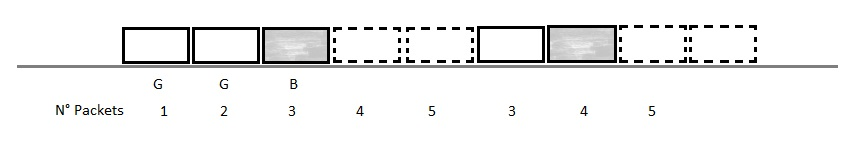
\includegraphics[width = .8\textwidth]{Cri_packets.jpg}
\caption{Go Back N scheme}
\label{fig:gbns}
\end{figure}
\begin{figure}
	\begin{center}
		\begin{tikzpicture}[->, >=stealth, auto, thin, node distance=3.5cm]
			\tikzstyle{every state}=[fill=white,draw=black,thin,text=black,scale=1]
			\node[state]		(G)											{$G$};
			\node[state]		(B)[right of=G]				{$B$};
			\path
			(G) 		edge[loop left]		 			node{$p_{00}$}				(G)
							edge[bend left]		 			node{$p_{01}$}		 		(B)
			(B)		edge[bend left]	node{$p_{01}(m)$}				(G)
							edge[loop right]					node{$p_{11}(m)$}	(B);

		\end{tikzpicture}
	\end{center}
	\caption{Graph model}
	\label{fig:GBN}
\end{figure}
In the model we can describe the behavior of the protocol like: \textit{If the slot is good, then go to the next one, otherwise skip $m-1$ slots and go to the $m^{th}$ one.}\\
With this reasoning it goes that the throughput is expressed as:
\beq
Throughput = \frac{\text{number of good slots}}{\text{total number of slots}}
\eeq
Every visit to state $G$ is $1$ success and every visit to state $B$ is a failure. The respective rewards are: $R_G = 1$ and $R_B = 0$; moreover we associate to $G$ and $B$ different time metrics: $T_{G} = 1$ and $T_{B} = m$, such that we obtain:
\beq
\lim_{t \to \infty}\frac{R(t)}{t} = \frac{\sum_i\pi_iR_i}{\sum_i\pi_iT_i}
\eeq
And the protocol chain is:
\beq
P =
\begin{bmatrix}
p_{00} & p_{01}\\
p_{10}(m) & p_{11}(m)
\end{bmatrix}
\eeq
To solve the limit we can find the $\pi$s like:
\begin{align}
\pi_{G} & = \frac{p_{10}(m)}{p_{10}(m)+p_{01}}\\
\pi_{B} & = \frac{p_{01}}{p_{10}(m)+p_{01}}
\end{align}
and insert them in the fraction, not considering the denominators, since they are the same for both the $\pi$s and so they would erase with each other.
\begin{align}
\begin{split}
\lim_{t \to \infty}\frac{R(t)}{t} & = \frac{\pi_GR_G+\pi_BR_B}{\pi_GT_G +\pi_BT_B}\\
& = \frac{p_{10}(m)\cdot1+p_{01}\cdot0}{p_{10}(m)\cdot1+p_{01}(m)}\\
& =\frac{p_{10}(m)}{p_{10}(m)+mp_{01}}
\end{split}
\end{align}
If we suppose an i.i.d. error we obtain:
\beq
\frac{1-\epsilon}{(1-\epsilon)+m\epsilon}
\eeq
Where $1-\epsilon$ is the \textit{P[having a good result | m previous results were bad]}, or better, \textit{P[having a good result]} since we hypothesized the independence of the errors.\\
Now let's try to answer another question: \textit{If we are in state G, how long does it take to us to come back?}\\
The answer is:
\beq
m_0 = p_{00}\cdot1+p_{01}[1+\frac{m}{p_{10}(m)}]
\label{Formula}
\eeq
Where $m_0$ is the average return time to $G$ and so the inverse of throughput; why? Because as in all semi-Markov processes, if we consider one state, visits to that one state are renewal instants. So the return time from $G$ to itself is a renewal interval and for this specific case, at every renewal cycle we have 1 success and the avg number of successes per unit time is the avg number of successes per cycle, $1$, divided by the average time per cycle. Moreover, once we have obtained the Markov structure we can identify the metrics we need to find.\\
Returning to the expression \eqref{Formula}, for the part  inside the rectangular brackets, the expression means that we stay in $B$ for a geometric number of times, which is equal to the average inverse outgoing probability. What we obtain after some algebra is:
\begin{align}
\begin{split}
m_0 & = 1+\frac{p_{01}\cdot m}{p_{10}(m)}\\
& = \frac{p_{10}(m)+mp_{01}}{p_{10}(m)}
\end{split}
\end{align}
\\
In the case the feedback has errors, we also need a M.C. for the acknowledgment and to combine it with the previous one, obtaining four states. But the only way to have successful transmission is that both the transmissions works fine:
\beq
C_f =
\begin{bmatrix}
p_{00} & p_{01}\\
p_{10} & p_{11}
\end{bmatrix}
\hspace{10mm}
C_b =
\begin{bmatrix}
q_{00} & q_{01}\\
q_{10} & q_{11}
\end{bmatrix}
\eeq
So the total transmission probability matrix is:
\beq
P =
\begin{bmatrix}
p_{00}q_{00} & p_{00}q_{01} & p_{01}q_{00} & p_{01}q_{01}\\
p_{00}(m)q_{10}(m) & p_{00}(m)q_{11}(m) & p_{01}(m)q_{10}(m) & p_{01}(m)q_{11}(m)\\
\text{$3^{rd}$ and} & \text{$4^{th}$ rows} & \text{can be} & \text{derived}\\
\text{in} & \text{a} & \text{similar} & \text{way}
\end{bmatrix}
\eeq
The state $00$ means $1$ success and $1$ slot, any other state is a failure: $0$ successes and $m$ slots. So I can rewrite the model, defining the vectors $R$ and $T$:
\beq
R =
\begin{bmatrix}
1\\
0\\
0\\
0
\end{bmatrix}
\hspace{20mm}
T =
\begin{bmatrix}
1\\
m\\
m\\
m
\end{bmatrix}
\eeq
and so obtaining the result:
\beq
\lim_{t \to \infty}\frac{R(t)}{t} = \frac{\bar{\pi}\bar{R}}{\bar{\pi}\bar{T}} = \frac{\pi_{00}\cdot 1}{\pi_{00}\cdot1+(1-\pi_{00})m}
\eeq
If now we suppose i.i.d. feedback errors w.p. $\delta$, we obtain the matrix
\beq
C_b =
\begin{bmatrix}
1-\delta & \delta\\
1-\delta & \delta
\end{bmatrix}
\eeq
Moreover, if the feedback channel is i.i.d., we have nothing to remember: regardless of whether the ack is good or bad, we do not care if the transmission was a failure $\rightarrow$ for this case we can use a simplified model with only $3$ states (figure\ref{fig:3states}), where the metrics are:
\beq
R =
\begin{bmatrix}
1\\
0\\
0
\end{bmatrix}
\hspace{5mm}
T =
\begin{bmatrix}
1\\
m\\
m
\end{bmatrix}
\eeq
\beq
p=
\begin{bmatrix}
(1-\delta)p_{00} & \delta p_{00} & p_{01}\\
(1-\delta)p{00}(m) & \delta p_{00}(m) & p_{01}(m)\\
(1-\delta)p_{10}(m) & \delta p_{10}(m) & p_{11}(m)
\end{bmatrix}
\eeq

\begin{figure}[h]
	\begin{center}
		\begin{tikzpicture}[->, >=stealth, auto, thin, node distance=4cm]
			\tikzstyle{every state}=[fill=white,draw=black,thin,text=black,scale=1]
			\node[state]		(G_0)											{$G_0$};
			\node[state]		(G_1)[below of=G]				{$G_1$};
			\node[state]		(B)[right of=G_1]		{$B$};
			\path
			(G_0) 	edge[loop left]	(G_0)
							edge[bend left=20]	(G_1)
							edge[bend left=20]	(B)
			(G_1)		edge[loop left]	(G_1)
							edge[bend left=20]	(G_0)
							edge[bend left=20]	(B)
			(B)			edge[loop right]	(B)
							edge[bend left=20]	(G_0)
							edge[bend left=20]	(G_1);
		\end{tikzpicture}
	\end{center}
	\caption{3-state model}
	\label{fig:3states}
\end{figure}
The throughput is:
\beq
\frac{\pi_{G_0}}{\pi_{G_0}+m(1-\pi_{G_0})}
\hspace{5mm}
\bar{\pi} = \bar{\pi}\cdot\bar{P}
\eeq
to obtain it we take:
\begin{align}
\pi_{G_0} & = (1-\delta)(\pi_{G_0}p_{00}+\pi_{G_1}p_{00}(m) +\pi_{B}p_{10}(m))\\
\pi_{G_1} & = \delta(\pi_{G_0}p_{00}+\pi_{G_1}p_{00}(m) +\pi_{B}p_{10}(m)) %Chiedere a Fede
\end{align}
where
\begin{itemize}
\item $(1-\delta)\pi_{G_1} = \delta\pi_{G_0}$
\item $(1-\delta)\pi_{B} = (1-\delta)-\pi_{G_0}$
\item $\pi_{B} = 1-\pi_{G_0}-\pi_{G_1} = 1-\pi_{G_0}-\frac{\delta}{1-\delta}\pi_{G_0} = 1- \frac{\pi_{G_0}}{1-\delta} = \frac{(1-\delta)-\pi_{G_0}}{1-\delta}$
\end{itemize}
and obtaining:
\begin{align}
\begin{split}
\pi_{G_0} & = (1-\delta)p_{00}\pi_{G_0} + \delta\pi_{G_0} p_{00}(m) (1-\delta-\pi_{G_0})p_{10}(m)\\
& = \frac{(1-\delta)p_{10}(m)}{1-(1-\delta)p_{00}-\delta p_{00}(m) +p_{10}(m)}
\end{split}
\end{align}
\beq
1-\pi_{G_0} = \frac{1-(1-\delta)p_{00} -\delta p_{00}(m) + \delta p_{10}(m)}{1-(1-\delta)p_{00}-\delta p_{00}(m) +p_{10}(m)}
\eeq
So the throughput is:
\beq
throughput = \frac{(1-\delta)p_{10}(m)}{(1-\delta)p_{10}(m) + m[1-(1-\delta)p_{00}-\delta p_{00}(m)+\delta p_{10}(m)]}
\eeq
\subsection{Graph reduction}
What if we rewrite the scheme, such that we can reduce it like in figure\ref{fig:GBN}?\\
From a memory point of view it is ok because we do not need to keep memory of the acknowledgments since they are i.i.d; but let's try to understand what happens in terms of success or failure of the acknowledgments:
\\
If we enter state $G$ (we tx a packet and it is succesful)we have:
\begin{itemize}
\item The ack is correct and we found $1$ success in $1$ slot w.p. $1-\delta$;
\item W.p. $\delta$ instead, we count $0$ successes in $m$ slots;
\end{itemize}
This brings us to conclude that in state $G$ we have:
\begin{itemize}
\item $1$ reward w.p. $1-\delta$, $0$ otherwise;
\item $1$ slot w.p. $1-\delta$, $m$ otherwise;
\end{itemize}
About transition probabilities:
\begin{itemize}
\item going to $G$ w.p. $(1-\delta)p_{00}+\delta p_{00}(m)$;
\item going to $B$ w.p. $(1-\delta)p_{01}+\delta p_{01}(m)$;
\end{itemize}
In state $B$ we have:
\begin{itemize}
\item No reward w.p. $1$ and $m$ slots always;
\item We go from there to $G$ w.p. $p_{10}(m)$;
\item And to $B$ w.p. $p_{11}(m)$;
\end{itemize}
So now we have a simplified Markov model where we combine into a single state everything that before was separate. What we obtain is:
\beq
\pi_{G} = \frac{p_{10}(m)}{(\dots)}
\hspace{20mm}
\pi_{B} = \frac{(1-\delta)p_{01}+\delta p_{01}(m)}{(\dots)}
\eeq
Reward and time:
\beq
R =
\begin{bmatrix}
1-\delta\\
0
\end{bmatrix}
\hspace{20mm}
T =
\begin{bmatrix}
1-\delta+\delta \cdot m\\
m
\end{bmatrix}
\eeq
And finally we can estimate the throughput for the system in figure\ref{fig:2states}:
\beq
\lim_{t \to \infty} \frac{R(t)}{t} = \frac{\bar{\pi}\bar{R}}{\bar{\pi}\bar{T}} = \frac{(1-\delta)p_{10}(m)}{(1-\delta+\delta \cdot m)p_{10}(m)+m[(1-\delta)p_{01}+\delta p_{01}(m)]}
\eeq
We just note that the denominator of this expression is equal to the one in the previous throughput expression: to prove it it is necessary to impose:
\begin{itemize}
\item $p_{00} = 1-p_{01}$;
\item $p_{00}(m) = 1-p_{01}(m)$
\end{itemize}
So $1-(1-\delta)p_{00}-\delta p_{00}(m) = (1-\delta)p_{01} + \delta p_{01}(m)$.\\
This result stands out from the fact that the two throughputs are the same quantity but computed by two different models; so we did not reduced the complexity, we just redistributed the quantities.
\begin{figure}[h]
	\begin{center}
		\begin{tikzpicture}[->, >=stealth, auto, thin, node distance=3.5cm]
			\tikzstyle{every state}=[fill=white,draw=black,thin,text=black,scale=1]
			\node[state]		(G)											{$G$};
			\node[state]		(B)[right of=G]				{$B$};
			\path
			(G) 		edge[loop left]		 			node{$(1-\delta)p_{00}+\delta p_{00}(m)$}				(G)
							edge[bend left=20]		 			node{$(1-\delta)p_{01} + \delta p_{01}(m)$}		 		(B)
			(B)		edge[bend left=20]	node{$p_{10}(m)$}				(G)
							edge[loop right]					node{$p_{11}(m)$}	(B);

		\end{tikzpicture}
	\end{center}
	\caption{2-state simplified model}
	\label{fig:2states}
\end{figure}
